%%%%%%%%%%%%%%%%%%%%%%%%%%%%%%%%%%%%%%%%%%%%%%%%%%%%%%%%%%%%%%%%%
%%% %
%%% % weiiszablon.tex
%%% % The Faculty of Electrical and Computer Engineering
%%% % Rzeszow University Of Technology diploma thesis Template
%%% % Szablon pracy dyplomowej Wydziału Elektrotechniki 
%%% % i Informatyki PRz
%%% % January, 2024
%%%%%%%%%%%%%%%%%%%%%%%%%%%%%%%%%%%%%%%%%%%%%%%%%%%%%%%%%%%%%%%%%

\documentclass[12pt,twoside]{article}

\usepackage{weiiszablon}

\author{Kacper Rychel}

% np. EF-123456, EN-654321, ...
\studentID{EF-173701}

\title{Robot mobilny z nawigacją autonomiczną oparty na Arduino}
\titleEN{Mobile robot with autonomous navigation based on Arduino}


%%% wybierz rodzaj pracy wpisując jeden z poniższych numerów: ...
% 1 = inżynierska	% BSc
% 2 = magisterska	% MSc
% 3 = doktorska		% PhD
% 4 = praca inżynierska
%%% na miejsce zera w linijce poniżej
\newcommand{\rodzajPracyNo}{1}


%%% promotor
\supervisor{Dr inż. Mariusz Mączka}
%% przykład: dr hab. inż. Józef Nowak, prof. PRz

%%% promotor ze stopniami naukowymi po angielsku
\supervisorEN{Prof. Mariusz Mączka}

\abstract{Cel pracy: Stworzenie robota mobilnego, który potrafi omijać przeszkody i poruszać się autonomicznie w środowisku. Zakres pracy: zaprojektowanie platformy robota z silnikami i czujnikami ultradźwiękowymi do detekcji przeszkód; zaprogramowanie algorytmu omijania przeszkód i nawigacji w środowisku; możliwość rozbudowy o funkcje śledzenia wyznaczonego celu lub powrotu do bazy. Testy robota w różnych scenariuszach, takich jak omijanie przeszkód czy poruszanie się po określonej trasie.}
\abstractEN{Objective: To create a mobile robot that can avoid obstacles and navigate autonomously within its environment. Scope of work: Designing a robot platform with motors and ultrasonic sensors for obstacle detection; programming an algorithm for obstacle avoidance and navigation within the environment; and the potential for expansion with target tracking or return-to-base functionality. Testing the robot in various scenarios, such as obstacle avoidance and navigating along a defined route.}

\keywords{Arduino Uno, Robot mobilny, Czujnik HC-SR04, Czujnik Ultradźwiękowy Odległości}
\keywordsEN{Arduino Uno, Mobile robot, HC-SR04 sensor, Ultrasonic distance sensor}


\begin{document}

% strona tytułowa
\maketitle

\blankpage

% spis treści
\tableofcontents

\clearpage
\blankpage

\section{Wprowadzenie}

Roboty mobilne należą do najbardziej dynamicznie rozwijających się obszarów współczesnej robotyki oraz inżynierii mechatronicznej. Ich znaczenie systematycznie rośnie wraz z postępem technologii obliczeniowych, czujnikowych oraz energetycznych, co przekłada się na coraz szerszy zakres zastosowań. Roboty mobilne wykorzystywane są obecnie m.in. w przemyśle, logistyce, eksploracji środowisk niebezpiecznych, a także w systemach autonomicznych. Zgodnie z definicją Międzynarodowej Federacji Robotyki, robot mobilny jest systemem mechatronicznym zdolnym do samodzielnego przemieszczania się w przestrzeni oraz realizacji określonych zadań bez stałego połączenia z infrastrukturą stacjonarną\cite{ifr2023}.

Rozwój mikrokontrolerów oraz popularyzacja platform open-source istotnie obniżyły próg wejścia w projektowaniu systemów robotycznych. Jak zauważa Monk, dostępność tanich i dobrze udokumentowanych platform, takich jak Arduino, umożliwia szybkie prototypowanie rozwiązań robotycznych również w warunkach edukacyjnych i amatorskich\cite{monk2016}. Dzięki temu możliwe stało się praktyczne łączenie zagadnień z zakresu elektroniki, programowania oraz automatyki w jednym projekcie.

Autonomia robota mobilnego rozumiana jest jako zdolność do samodzielnego podejmowania decyzji na podstawie informacji pozyskiwanych z czujników. System autonomiczny integruje procesy percepcji otoczenia, podejmowania decyzji oraz sterowania ruchem. Siegwart, Nourbakhsh i Scaramuzza wskazują, że nawet w przypadku prostych algorytmów reaktywnych niezbędna jest spójna współpraca tych elementów, aby robot mógł funkcjonować w sposób przewidywalny i bezpieczny\cite{siegwart2011}.

Centralnym elementem sterującym robota mobilnego jest mikrokontroler, odpowiedzialny za przetwarzanie danych sensorycznych oraz generowanie sygnałów sterujących elementami wykonawczymi. Platforma Arduino UNO, oparta na mikrokontrolerze ATmega328P, należy do najczęściej wykorzystywanych w projektach edukacyjnych ze względu na bogatą dokumentację techniczną, dostępność bibliotek programistycznych oraz szerokie wsparcie społeczności open-source\cite{arduino2022}. Zastosowanie gotowych bibliotek znacząco skraca czas implementacji algorytmów sterowania oraz obsługi czujników.

Istotną rolę w systemach autonomicznych odgrywają czujniki umożliwiające pozyskiwanie informacji o otoczeniu. W robotach niskokosztowych powszechnie wykorzystuje się czujniki ultradźwiękowe, które pozwalają na pomiar odległości na podstawie czasu przelotu fali akustycznej. Popularnym rozwiązaniem w projektach edukacyjnych jest moduł HC-SR04, który charakteryzuje się niewielkim kosztem, prostą obsługą oraz łatwą integracją z mikrokontrolerami\cite{elecfreaks}. Dokumentacja producenta wskazuje, że dokładność pomiaru jest wystarczająca dla podstawowych algorytmów nawigacyjnych, choć należy uwzględnić wpływ właściwości powierzchni odbijających oraz warunków środowiskowych\cite{cytron2018}.

Ruch robota mobilnego realizowany jest najczęściej za pomocą napędu różnicowego, składającego się z dwóch niezależnie sterowanych silników prądu stałego. Taki układ umożliwia realizację manewrów poprzez różnicowanie prędkości obrotowych kół. Jak wskazują Jones, Flynn i Seiger, napęd różnicowy cechuje się niewielką złożonością mechaniczną i sterowniczą, co czyni go jednym z najczęściej stosowanych rozwiązań w robotach mobilnych\cite{jones1999}. Do sterowania silnikami prądu stałego stosuje się układy typu mostek H, takie jak L293D, umożliwiające zmianę kierunku obrotów oraz regulację prędkości z wykorzystaniem sygnału PWM. Tego typu układy stanowią podstawowy element wykonawczy w systemach sterowania napędami niskiej mocy\cite{horowitz2015}.

Praca podzielona jest na trzy rozdziały. W drugim rozdziale przedstawiony jest zakres teoretyczny zagadnień potrzebnych do skompletowania robota. Trzeci rozdział przeznaczony jest skupieniu najważniejszych elementów budowania fizycznej podstawy robota. W czwartym rozdziale opisany został kod programowy robota.
 
Celem niniejszej pracy jest zaprojektowanie i wykonanie autonomicznego robota mobilnego opartego na platformie Arduino UNO, zdolnego do samodzielnego poruszania się oraz unikania przeszkód na podstawie pomiarów odległości. Zakres pracy obejmuje analizę teoretyczną zagadnień robotyki mobilnej, projekt i realizację układu sprzętowego, implementację algorytmu sterowania oraz przeprowadzenie testów funkcjonalnych opracowanego rozwiązania.

\section{Zakres teoretyczny z dziedziny robotyki}

Coś tam

\subsection{Przegląd stanu wiedzy i techniki w zakresie robotów mobilnych}

Postęp technologiczny w obszarze robotyki mobilnej, obserwowany w ostatnich dekadach, doprowadził do wykształcenia się wielu zróżnicowanych podejść konstrukcyjnych oraz algorytmicznych. Dobór konkretnego rozwiązania zależy przede wszystkim od przeznaczenia robota, charakterystyki środowiska pracy oraz dostępnych zasobów sprzętowych i obliczeniowych. Jak podkreśla się w literaturze przedmiotu, pomimo dynamicznego rozwoju systemów autonomicznych i algorytmów sztucznej inteligencji, w dalszym ciągu istotną rolę odgrywają rozwiązania proste i deterministyczne, szczególnie w systemach o charakterze edukacyjnym oraz prototypowym \cite{educationalRoboticsOverview}.

\subsubsection{Modelowanie ruchu robota}

Jednym z podstawowych zagadnień w robotyce mobilnej jest modelowanie ruchu robota, stanowiące fundament projektowania algorytmów sterowania oraz nawigacji. W przypadku najczęściej spotykanego napędu różnicowego ruch robota opisywany jest za pomocą nieliniowego modelu kinematycznego, w którym prędkość liniowa oraz prędkość kątowa platformy są bezpośrednio zależne od prędkości obrotowych kół napędowych. Campion, Bastin oraz D’Andrea-Novel wskazują, że model kinematyczny robota z napędem różnicowym cechuje się prostotą implementacji, jednak wprowadza istotne ograniczenie w postaci braku możliwości realizacji ruchu bocznego\cite{campionDifferentialDrive}. Ograniczenie to wymusza stosowanie odpowiednich strategii planowania trajektorii oraz manewrowania, zwłaszcza w środowiskach o ograniczonej przestrzeni roboczej.

W praktycznych realizacjach robotów mobilnych, szczególnie w systemach dysponujących niewielką mocą obliczeniową, sterowanie ruchem realizowane jest zazwyczaj w oparciu o regulatory dyskretne, bez jawnego uwzględniania pełnego modelu dynamicznego. Regulacja prędkości silników prądu stałego odbywa się najczęściej przy użyciu modulacji szerokości impulsu PWM, natomiast zmiana kierunku obrotów realizowana jest poprzez odpowiednie sterowanie mostkiem H. Jak zauważają Horowitz i Hill, takie podejście, mimo swojej prostoty, jest w pełni wystarczające w systemach, w których nie jest wymagana wysoka precyzja pozycjonowania ani zaawansowana regulacja momentu obrotowego\cite{horowitz2015}.

\subsubsection{Odtwarzanie danych sensorycznych}

Istotnym elementem wpływającym na skuteczność autonomii robota mobilnego jest sposób pozyskiwania oraz przetwarzania danych sensorycznych. W systemach niskokosztowych dominują rozwiązania wykorzystujące pojedyncze lub kilka czujników odległości, których wskazania są bezpośrednio wykorzystywane do podejmowania decyzji ruchowych. Takie podejście określane jest w literaturze mianem nawigacji reaktywnej, w której robot nie buduje globalnej reprezentacji środowiska, lecz reaguje wyłącznie na aktualnie wykryte przeszkody\cite{reactiveNavigation}. Metody te, choć nieoptymalne z punktu widzenia długości trajektorii czy efektywności ruchu, charakteryzują się dużą odpornością na zmiany otoczenia oraz niewielkimi wymaganiami obliczeniowymi.

W algorytmach nawigacji reaktywnej powszechnie stosowane są czujniki ultradźwiękowe, cenione za prostą zasadę działania oraz łatwość integracji z popularnymi mikrokontrolerami. Badania porównawcze czujników odległości wskazują, że dokładność pomiarów ultradźwiękowych jest wystarczająca do wykrywania przeszkód o rozmiarach porównywalnych z wymiarami robota, jednak ulega pogorszeniu w przypadku powierzchni pochłaniających fale akustyczne lub ustawionych pod znacznym kątem względem osi pomiaru\cite{ultrasonicSensorComparison}. Z tego względu zaleca się stosowanie odpowiednich marginesów bezpieczeństwa w algorytmach decyzyjnych oraz filtrację wyników pomiarów w celu zwiększenia odporności systemu na błędne odczyty\cite{sensorFiltering}.

\subsubsection{Technologia mapowania SLAM}
W bardziej zaawansowanych systemach robotów mobilnych stosowane są techniki lokalizacji i mapowania jednoczesnego (SLAM), wykorzystujące dane z czujników LiDARowych\footnote{LiDAR (Light Detection and Ranging) - metoda pomiarowa używana do określania precyzyjnego dystansu obiektu.}, kamer wizyjnych oraz jednostek inercyjnych. Metody te umożliwiają jednoczesną budowę mapy otoczenia oraz precyzyjne określanie położenia robota, jednak wiążą się z wysokimi wymaganiami obliczeniowymi oraz znaczną złożonością implementacyjną\cite{slamOverview}. Jak podkreśla Thrun, implementacja algorytmów SLAM w systemach edukacyjnych jest często nieuzasadniona, gdyż poziom skomplikowania może przesłaniać podstawowe zagadnienia inżynierskie, takie jak sterowanie ruchem czy integracja czujników\cite{thrunSLAM}.

\subsection{Klasyfikacja i architektura robotów mobilnych}

Roboty mobilne mogą być klasyfikowane według wielu różnych kryteriów, co wynika z dużej różnorodności ich konstrukcji, przeznaczenia oraz środowisk pracy. W literaturze przedmiotu podkreśla się, że brak jednej uniwersalnej klasyfikacji robotów mobilnych jest konsekwencją interdyscyplinarnego charakteru tej dziedziny, łączącej zagadnienia z zakresu mechaniki, elektroniki, informatyki oraz teorii sterowania\cite{mobileRoboticsClassification}. Najczęściej spotykane podejścia klasyfikacyjne obejmują podział ze względu na mechanizm lokomocji, stopień autonomii, środowisko eksploatacji oraz zakres realizowanych zadań.

\subsubsection{Klasyfikacja według sposobu lokomocji robota}

Jednym z podstawowych i najbardziej intuicyjnych kryteriów klasyfikacji robotów mobilnych jest sposób ich poruszania się. W tym ujęciu wyróżnia się roboty kołowe, gąsienicowe, kroczące oraz konstrukcje hybrydowe. Roboty kołowe, wyposażone w jedno lub więcej kół napędowych, charakteryzują się wysoką sprawnością energetyczną, niewielkimi stratami energii wynikającymi z oporów toczenia oraz prostotą konstrukcji mechanicznej. Jak wskazuje Siegwart, łatwość sterowania oraz stosunkowo niski koszt wykonania sprawiają, że roboty kołowe dominują w zastosowaniach edukacyjnych, przemysłowych oraz badawczych\cite{siegwart2011}. Ich istotnym ograniczeniem jest jednak ograniczona zdolność poruszania się po nierównym lub nieuporządkowanym terenie, co zawęża zakres potencjalnych zastosowań.

Alternatywę dla konstrukcji kołowych stanowią roboty gąsienicowe, które dzięki większej powierzchni styku z podłożem cechują się lepszą przyczepnością oraz zdolnością pokonywania przeszkód terenowych. Z tego względu znajdują one zastosowanie w robotach eksploracyjnych, ratowniczych oraz wojskowych, gdzie wymagana jest wysoka stabilność ruchu w trudnych warunkach środowiskowych. Jak zauważa Borenstein, zwiększone opory ruchu oraz większa złożoność mechaniczna układów gąsienicowych prowadzą do wyższego zużycia energii oraz utrudniają precyzyjne sterowanie ruchem w porównaniu z robotami kołowymi\cite{borensteinMobilePlatforms}.

Najbardziej złożoną grupę robotów mobilnych pod względem konstrukcyjnym i algorytmicznym stanowią roboty kroczące. Ich lokomocja opiera się na sekwencyjnym przemieszczaniu kończyn, co umożliwia poruszanie się w terenie niedostępnym dla robotów kołowych i gąsienicowych, takim jak schody, gruzowiska czy obszary o znacznych nierównościach. Projektowanie robotów kroczących wymaga zaawansowanego modelowania dynamiki, precyzyjnego sterowania ruchem oraz znacznych zasobów obliczeniowych\cite{leggedRobotsControl}.

\subsubsection{Klasyfikacja według autonomiczności robota}

Istotnym kryterium klasyfikacji robotów mobilnych, niezależnym od mechanizmu lokomocji, jest stopień autonomii systemu. W tym ujęciu wyróżnia się roboty zdalnie sterowane, półautonomiczne oraz autonomiczne. Roboty zdalnie sterowane wymagają stałej ingerencji operatora i nie podejmują samodzielnych decyzji, roboty autonomiczne są zdolne do samodzielnej analizy danych sensorycznych, planowania działań oraz realizacji zadań bez bezpośredniego nadzoru człowieka, natomiast roboty półautonomiczne są hybrydowym rozwiązaniem łączącym cechy maszyn autonomicznych oraz zdalnie sterowanych. Jak wskazuje Arkin, poziom autonomii robota jest ściśle powiązany z zastosowanymi algorytmami decyzyjnymi oraz architekturą systemu sterowania\cite{reactiveNavigation}.

\subsubsection{Klasyfikacja według architektury rozwiązania}

Z punktu widzenia architektury systemowej robot mobilny stanowi złożony system mechatroniczny, który można opisać jako zbiór współpracujących ze sobą warstw funkcjonalnych. Wyróżnia się warstwę sensoryczną, odpowiedzialną za pozyskiwanie informacji o stanie robota i jego otoczeniu, warstwę decyzyjną, w której realizowane są algorytmy sterowania i nawigacji, oraz warstwę wykonawczą, obejmującą układy napędowe i elementy wykonawcze. Taki podział funkcjonalny jest powszechnie stosowany w literaturze i umożliwia modularne oraz skalowalne projektowanie systemów robotycznych\cite{jones1999}.

Warstwa sensoryczna obejmuje zestaw czujników, takich jak czujniki odległości, enkodery, czujniki inercyjne czy kamery wizyjne, których zadaniem jest dostarczanie informacji o położeniu robota, jego ruchu oraz otoczeniu. Rodzaj i jakość danych sensorycznych w istotny sposób wpływają na możliwości percepcyjne systemu oraz skuteczność podejmowanych decyzji.

Warstwa decyzyjna stanowi centralny element architektury robota mobilnego. W prostych konstrukcjach realizowana jest bezpośrednio na mikrokontrolerze, który przetwarza dane sensoryczne i generuje sygnały sterujące w czasie rzeczywistym. W bardziej zaawansowanych systemach warstwa ta może być rozproszona pomiędzy kilka jednostek obliczeniowych, takich jak komputery jednopłytkowe lub procesory dedykowane, co umożliwia implementację złożonych algorytmów planowania trajektorii, lokalizacji czy uczenia maszynowego\cite{advancedRobotArchitectures}. Rozwiązania te zwiększają jednak złożoność systemu oraz zapotrzebowanie na energię.

Warstwa wykonawcza obejmuje elementy odpowiedzialne za fizyczną realizację ruchu robota, w tym silniki, przekładnie mechaniczne oraz układy sterujące. Jej projekt musi uwzględniać wymagania mechaniczne i elektryczne, a także ograniczenia wynikające z zastosowanego źródła zasilania. Jak podkreślają Jones i Flynn, prawidłowa integracja warstwy wykonawczej z pozostałymi warstwami systemu jest kluczowa dla zapewnienia stabilnego, przewidywalnego i bezpiecznego zachowania robota mobilnego\cite{jones1999}.

\subsection{Modelowanie ruchu robotów mobilnych}

Modelowanie ruchu robota mobilnego stanowi jeden z kluczowych etapów projektowania systemów sterowania oraz nawigacji, gdyż umożliwia formalny, matematyczny opis zależności pomiędzy sygnałami sterującymi a rzeczywistym ruchem platformy. W robotyce mobilnej wyróżnia się dwa podstawowe podejścia do opisu ruchu: modelowanie kinematyczne oraz dynamiczne. Model kinematyczny koncentruje się na zależnościach geometrycznych i prędkościowych, pomijając wpływ sił oraz momentów działających na robota, natomiast model dynamiczny uwzględnia masę, bezwładność oraz oddziaływania z otoczeniem\cite{robotKinematicsDynamics}. W przypadku większości robotów edukacyjnych i prototypowych stosuje się modele kinematyczne, które zapewniają wystarczającą dokładność przy znacznie mniejszej złożoności obliczeniowej.

Najczęściej spotykanym rozwiązaniem konstrukcyjnym w robotach mobilnych jest napęd różnicowy, składający się z dwóch niezależnie sterowanych kół napędowych umieszczonych po przeciwnych stronach platformy oraz jednego lub więcej elementów podparcia biernego. Ruch robota wyposażonego w taki napęd może być opisany za pomocą zestawu równań kinematycznych, w których prędkość liniowa oraz prędkość kątowa platformy są bezpośrednią funkcją prędkości obrotowych lewego i prawego koła. Model ten cechuje się prostotą formalną oraz intuicyjnością, co czyni go szczególnie przydatnym w projektach dydaktycznych oraz na wczesnych etapach prototypowania\cite{campionDifferentialDrive}.

Formalny opis kinematyki robota z napędem różnicowym prowadzi do nieliniowego układu równań, w którym pozycja robota opisywana jest zazwyczaj za pomocą współrzędnych płaskich oraz kąta orientacji względem przyjętego układu odniesienia. Nieliniowość modelu wynika z faktu, że orientacja robota wpływa bezpośrednio na kierunek jego ruchu postępowego. W praktyce oznacza to konieczność ciągłego uwzględniania aktualnego położenia i orientacji robota podczas sterowania ruchem, nawet w przypadku realizacji prostych manewrów, takich jak jazda po łuku lub zmiana kierunku jazdy\cite{mobileRobotNonlinearModel}.

Istotnym ograniczeniem wynikającym z kinematyki napędu różnicowego jest brak możliwości realizacji ruchu bocznego. Robot nie jest w stanie przemieszczać się w kierunku prostopadłym do osi swojej orientacji bez wcześniejszego wykonania obrotu. W literaturze ograniczenia tego typu określane są mianem ograniczeń nieholonomicznych i mają one istotny wpływ na projektowanie algorytmów sterowania oraz nawigacji\cite{nonholonomicConstraints}. Ograniczenia nieholonomiczne powodują, że trajektorie ruchu robota muszą spełniać określone warunki ciągłości i gładkości, co komplikuje planowanie ruchu w środowiskach o ograniczonej przestrzeni.

Konsekwencją występowania ograniczeń nieholonomicznych jest konieczność stosowania odpowiednich strategii manewrowania, szczególnie podczas omijania przeszkód. W prostych systemach autonomicznych często wykorzystuje się sekwencje ruchów elementarnych, takich jak jazda do przodu, obrót w miejscu oraz cofanie, które w połączeniu umożliwiają realizację bardziej złożonych manewrów. Jak podkreśla Thrun, takie podejście jest wystarczające w środowiskach o niewielkiej złożoności i stanowi rozsądny kompromis pomiędzy prostotą implementacji a funkcjonalnością systemu\cite{thrunSLAM}.

W praktycznych realizacjach robotów mobilnych model kinematyczny wykorzystywany jest głównie pośrednio, jako podstawa do projektowania algorytmów sterowania niskiego poziomu. Zamiast ciągłego rozwiązywania równań ruchu stosuje się sterowanie dyskretne, w którym decyzje podejmowane są w kolejnych krokach czasowych na podstawie aktualnych danych sensorycznych. Takie podejście jest szczególnie korzystne w systemach opartych na mikrokontrolerach o ograniczonej mocy obliczeniowej, gdzie kluczowe znaczenie ma krótki czas reakcji oraz stabilność działania\cite{embeddedMotorControl}.

W literaturze podkreśla się również, że w robotach edukacyjnych dokładność modelu kinematycznego ma często znaczenie drugorzędne w porównaniu z jego czytelnością i łatwością interpretacji. Błędy wynikające z poślizgu kół, nierówności podłoża czy niedokładności wykonania mechanicznego są zazwyczaj akceptowalne, o ile algorytm sterowania wykazuje odpowiednią odporność na zakłócenia\cite{educationalRobotsModeling}. Z tego względu w wielu konstrukcjach rezygnuje się z enkoderów oraz sprzężenia zwrotnego pozycji na rzecz prostych algorytmów otwartej pętli, opartych na czasie trwania ruchu oraz zadanej prędkości.

Ograniczenia kinematyczne robotów kołowych mają również bezpośredni wpływ na sposób planowania trajektorii. W systemach o wyższym stopniu zaawansowania stosuje się algorytmy planowania ruchu uwzględniające nieholonomiczność, takie jak planowanie w przestrzeni konfiguracyjnej czy metody oparte na krzywych Dubinsa. Jak zauważa LaValle, metody te wymagają precyzyjnego modelu robota oraz znacznych zasobów obliczeniowych, co w praktyce ogranicza ich zastosowanie w prostych platformach mobilnych\cite{lavallePlanningAlgorithms}.

Z tego względu w systemach o charakterze edukacyjnym i prototypowym często rezygnuje się z planowania globalnego na rzecz lokalnych algorytmów decyzyjnych, bazujących na bieżących pomiarach sensorycznych. Podejście to, mimo że nie gwarantuje optymalności trajektorii, umożliwia skuteczne poruszanie się robota w nieznanym środowisku i jest zgodne z ograniczeniami sprzętowymi oraz obliczeniowymi prostych platform mobilnych.


\subsection{Układy napędowe i sterowanie silnikami}

Układ napędowy robota mobilnego stanowi podstawowy element warstwy wykonawczej systemu, bezpośrednio odpowiedzialny za realizację poleceń generowanych przez warstwę decyzyjną. Jego zadaniem jest przekształcenie sygnałów sterujących w rzeczywisty ruch platformy przy zachowaniu możliwie wysokiej sprawności energetycznej, stabilności działania oraz przewidywalnego zachowania robota. W praktycznych realizacjach robotów mobilnych, najczęściej stosowane są silniki prądu stałego z magnesami trwałymi, które łączą prostotę sterowania z korzystnymi parametrami mechanicznymi i niewielkimi wymaganiami sprzętowymi.

Silniki prądu stałego charakteryzują się w przybliżeniu liniową zależnością momentu obrotowego od prądu twornika oraz zależnością prędkości obrotowej od napięcia zasilania. Właściwości te umożliwiają stosunkowo łatwą regulację prędkości obrotowej bez konieczności stosowania złożonych algorytmów regulacji. W robotach mobilnych silniki te zazwyczaj współpracują z przekładniami redukcyjnymi, które zwiększają dostępny moment obrotowy kosztem prędkości.

Regulacja prędkości obrotowej silników prądu stałego realizowana jest najczęściej przy wykorzystaniu modulacji szerokości impulsu PWM (Pulse Width Modulation). Metoda ta polega na okresowym załączaniu i wyłączaniu napięcia zasilającego silnik z ustaloną częstotliwością oraz zmiennym współczynnikiem wypełnienia. Ze względu na indukcyjność uzwojeń silnika oraz jego bezwładność mechaniczną sygnał PWM postrzegany jest jako napięcie o wartości średniej proporcjonalnej do wypełnienia impulsu. Jak podkreślają Horowitz i Hill, modulacja PWM umożliwia efektywną regulację prędkości przy minimalnych stratach mocy, co czyni ją standardowym rozwiązaniem w systemach sterowania napędami niskonapięciowymi\cite{horowitz2015}.

Istotnym zagadnieniem w sterowaniu napędem robota mobilnego jest możliwość zmiany kierunku obrotów silnika. Wymaga to zastosowania układu umożliwiającego odwrócenie polaryzacji napięcia zasilającego, co najczęściej realizowane jest za pomocą mostka H. Układ ten składa się z zestawu elementów przełączających, takich jak tranzystory bipolarne lub MOSFET\footnote{MOSFET - podstawowa technologia produkcji większości półprzewodników z izolowaną bramką stosowanych w komputerach.}, które pozwalają na sterowanie kierunkiem przepływu prądu przez silnik. W rozwiązaniach edukacyjnych powszechnie stosowane są scalone układy mostków H, integrujące elementy mocy oraz podstawowe zabezpieczenia w jednej obudowie.

Jednym z najczęściej wykorzystywanych układów tego typu jest L293D, który umożliwia niezależne sterowanie dwoma silnikami prądu stałego. Układ ten pozwala na realizację zmiany kierunku obrotów poprzez odpowiednie stany logiczne na wejściach sterujących, natomiast regulacja prędkości realizowana jest przez doprowadzenie sygnału PWM do wejścia aktywującego. Takie rozwiązanie jest szczególnie korzystne, gdyż umożliwia prostą i czytelną implementację sterowania ruchem bez konieczności projektowania własnych układów mocy.

W robotach mobilnych o niewielkich rozmiarach istotne znaczenie ma również sposób zasilania układu napędowego. Silniki prądu stałego charakteryzują się stosunkowo dużymi prądami rozruchowymi, które mogą prowadzić do chwilowych spadków napięcia oraz zakłóceń pracy układów logicznych. Z tego względu w literaturze zaleca się separację zasilania części wykonawczej i logicznej lub stosowanie odpowiednich filtrów oraz kondensatorów buforujących\cite{motorPowerSupplyIssues}. W prostych konstrukcjach edukacyjnych zagadnienie to bywa często pomijane, jednak jego uwzględnienie znacząco poprawia stabilność i niezawodność całego systemu.

\subsubsection{Sterowanie silnikami robota}

Sterowanie silnikami w robotach mobilnych może być realizowane zarówno w pętli otwartej, jak i zamkniętej. W systemach edukacyjnych i prototypowych dominującym rozwiązaniem jest sterowanie w pętli otwartej, w którym prędkość oraz czas trwania ruchu ustalane są na podstawie zadanych wartości sygnału PWM. Brak sprzężenia zwrotnego z enkoderów oznacza, że system nie kompensuje odchyłek wynikających z poślizgu kół, nierówności podłoża czy różnic parametrów silników. Jak zauważają Horowitz i Hill, w wielu zastosowaniach tego typu uproszczenie jest w pełni akceptowalne i nie wpływa istotnie na funkcjonalność systemu \cite{horowitz2015}.

W bardziej zaawansowanych konstrukcjach stosuje się enkodery obrotowe, które umożliwiają pomiar prędkości oraz kąta obrotu kół. Pozwala to na implementację regulatorów prędkości, najczęściej typu PID, oraz na dokładniejsze sterowanie ruchem robota. Należy jednak podkreślić, że zastosowanie sprzężenia zwrotnego wiąże się ze wzrostem złożoności zarówno sprzętowej, jak i programowej, co może być niepożądane w projektach o charakterze dydaktycznym.

Z punktu widzenia architektury systemowej układ napędowy stanowi interfejs pomiędzy warstwą decyzyjną a fizycznym ruchem robota. Prostota jego realizacji ma istotne znaczenie dla przejrzystości projektu oraz możliwości dalszej rozbudowy systemu. W konstrukcjach opartych na mikrokontrolerach, takich jak Arduino, wykorzystanie standardowych bibliotek do obsługi PWM oraz gotowych sterowników silników pozwala skoncentrować się na zagadnieniach algorytmicznych, zamiast na niskopoziomowych detalach sprzętowych.

\subsection{Percepcja otoczenia}

Percepcja otoczenia stanowi jeden z fundamentalnych elementów autonomii robota mobilnego, gdyż to na jej podstawie system podejmuje decyzje dotyczące ruchu oraz reakcji na zmieniające się warunki środowiskowe. W przeciwieństwie do systemów sterowanych zdalnie, robot autonomiczny musi samodzielnie interpretować sygnały pochodzące z czujników i przekształcać je w działania zgodne z przyjętą strategią sterowania. W literaturze podkreśla się, że jakość procesu percepcji ma bezpośredni wpływ na bezpieczeństwo oraz skuteczność poruszania się robota, niezależnie od stopnia zaawansowania zastosowanych algorytmów decyzyjnych\cite{jones1999}.

Wśród czujników wykorzystywanych w systemach reaktywnych szczególnie szerokie zastosowanie znajdują czujniki ultradźwiękowe. Ich zasada działania polega na emisji krótkiego impulsu fali akustycznej o wysokiej częstotliwości oraz pomiarze czasu, po którym sygnał powraca do odbiornika po odbiciu od przeszkody. Znając prędkość rozchodzenia się dźwięku w powietrzu, możliwe jest wyznaczenie odległości do obiektu.

Badania porównawcze czujników odległości wskazują, że czujniki ultradźwiękowe zapewniają wystarczającą dokładność pomiaru dla podstawowych zadań unikania przeszkód, szczególnie w zakresie odległości od kilkunastu do kilkudziesięciu centymetrów\cite{ultrasonicSensorComparison}. Skuteczność tych czujników zależy jednak w dużym stopniu od właściwości powierzchni odbijającej falę akustyczną. Powierzchnie miękkie, porowate lub ustawione pod znacznym kątem względem osi pomiaru mogą powodować osłabienie lub rozproszenie sygnału odbitego, prowadząc do błędnych odczytów. Na dokładność pomiarów wpływają również warunki środowiskowe, takie jak temperatura powietrza czy obecność zakłóceń akustycznych.

Z tego względu istotnym elementem przetwarzania danych sensorycznych jest odpowiednia filtracja wyników pomiarów. W prostych systemach stosuje się najczęściej uśrednianie kilku kolejnych odczytów lub odrzucanie wartości skrajnych, które mogą być skutkiem chwilowych zakłóceń. Zaleca się także wprowadzanie progów decyzyjnych, zwiększających odporność algorytmu sterowania na pojedyncze błędne pomiary\cite{sensorFiltering}. Przykładowo, decyzja o zmianie kierunku ruchu może być podejmowana dopiero po kilkukrotnym potwierdzeniu obecności przeszkody w określonym zakresie odległości.

W bardziej rozbudowanych rozwiązaniach możliwe jest łączenie danych pochodzących z kilku czujników odległości, rozmieszczonych w różnych kierunkach wokół robota. Takie podejście pozwala na uzyskanie bardziej kompletnej informacji o otoczeniu bez konieczności stosowania zaawansowanych czujników. Integracja wielu źródeł danych sensorycznych, określana mianem fuzji sensorycznej, może istotnie zwiększyć niezawodność procesu percepcji, jednak wiąże się ze wzrostem złożoności algorytmów decyzyjnych oraz wymaga starannego doboru parametrów czasowych.

W kontekście mikrokontrolerów, takich jak Arduino UNO, przetwarzanie danych sensorycznych musi być realizowane w sposób efektywny czasowo. Pomiar odległości z wykorzystaniem czujnika ultradźwiękowego wymaga precyzyjnego odmierzania czasu trwania impulsu powrotnego, co realizowane jest z wykorzystaniem liczników sprzętowych lub mechanizmów przerwań. Odpowiednia organizacja programu, obejmująca cykliczny odczyt czujników oraz sekwencyjne podejmowanie decyzji, ma kolosalne znaczenie dla zapewnienia reakcji robota w czasie zbliżonym do rzeczywistego.

Należy również zwrócić uwagę na kompromis pomiędzy częstotliwością odczytu czujników a stabilnością działania algorytmu sterowania. Zbyt częste pomiary mogą prowadzić do nadmiernej liczby decyzji ruchowych i niestabilności toru jazdy, natomiast zbyt rzadkie odczyty zwiększają ryzyko kolizji z przeszkodami. W literaturze podkreśla się konieczność doboru parametrów czasowych w sposób dostosowany do prędkości robota oraz dynamiki środowiska pracy.

\subsection{Zaawansowane metody nawigacji}

Postęp w zakresie mocy obliczeniowej systemów wbudowanych oraz rosnąca dostępność zaawansowanych czujników pomiarowych przyczyniły się do dynamicznego rozwoju metod lokalizacji i nawigacji robotów mobilnych. W odróżnieniu od podejść reaktywnych, które bazują wyłącznie na bieżących pomiarach sensorycznych, metody zaawansowane zakładają istnienie wewnętrznej reprezentacji środowiska oraz ciągłą estymację położenia robota w czasie. Centralnym zagadnieniem w tym obszarze jest problem jednoczesnej lokalizacji i mapowania, znany w literaturze jako SLAM (Simultaneous Localization and Mapping).

Algorytmy SLAM umożliwiają stopniowe tworzenie mapy nieznanego środowiska przy jednoczesnym określaniu pozycji robota względem tej mapy. Złożoność tego problemu wynika z faktu, że zarówno dane sensoryczne, jak i modele ruchu obarczone są niepewnością, której kumulacja prowadzi do narastania błędów lokalizacji. Jak podkreśla Thrun, SLAM stanowi jedno z fundamentalnych wyzwań współczesnej robotyki mobilnej, łącząc elementy probabilistyki, estymacji stanu oraz sztucznej inteligencji \cite{thrunSLAM}.

W praktycznych implementacjach algorytmy SLAM wykorzystują dane pochodzące z wielu źródeł sensorycznych. Najczęściej stosowane są czujniki LiDARowe, dostarczające precyzyjnych informacji o geometrii otoczenia, kamery wizyjne umożliwiające analizę cech wizualnych środowiska oraz jednostki inercyjne, pozwalające na estymację przyspieszeń i prędkości kątowych robota. Fuzja danych z różnych czujników zwiększa dokładność lokalizacji oraz poprawia odporność systemu na zakłócenia lub chwilową utratę sygnału z jednego z kanałów pomiarowych\cite{siegwart2011}.

W literaturze wyróżnia się kilka klas algorytmów SLAM, różniących się sposobem reprezentacji niepewności oraz złożonością obliczeniową. Do najwcześniej stosowanych należą metody oparte na filtrze Kalmana oraz jego rozszerzeniach, takich jak rozszerzony filtr Kalmana (EKF), które znajdują zastosowanie głównie w systemach o ograniczonej liczbie stanów. Algorytmy cząsteczkowe, w tym FastSLAM, umożliwiają lepsze odwzorowanie nieliniowości oraz wielomodalności rozkładów prawdopodobieństwa, jednak wiążą się ze znacznym wzrostem zapotrzebowania na moc obliczeniową. W nowoczesnych systemach autonomicznych coraz częściej stosuje się metody grafowe, charakteryzujące się wysoką dokładnością estymacji, kosztem złożonej implementacji oraz dużych wymagań sprzętowych.

Poza lokalizacją i mapowaniem istotnym elementem zaawansowanej nawigacji jest planowanie ruchu. W systemach dysponujących mapą środowiska wykorzystuje się algorytmy planowania globalnego, których zadaniem jest wyznaczenie trajektorii pomiędzy pozycją początkową a celem. Do najczęściej stosowanych należą algorytmy grafowe, takie jak Dijkstra czy A*, a także algorytmy losowe, w tym RRT (Rapidly-exploring Random Trees). Planowanie globalne umożliwia efektywne omijanie przeszkód oraz minimalizację długości trajektorii, jednak jego skuteczność jest ściśle uzależniona od jakości mapy oraz dokładności lokalizacji robota\cite{siegwart2011}.

Uzupełnieniem planowania globalnego są algorytmy planowania lokalnego, odpowiedzialne za reagowanie na dynamiczne zmiany w otoczeniu, takie jak pojawienie się przeszkód ruchomych lub nieprzewidziane zakłócenia. W praktycznych systemach autonomicznych często stosuje się architektury hybrydowe, w których plan globalny stanowi punkt odniesienia, natomiast algorytmy lokalne realizują bieżącą korektę ruchu. Takie podejście zwiększa skuteczność działania robota w złożonych środowiskach, lecz jednocześnie prowadzi do znacznego wzrostu złożoności całego systemu sterowania.

Pomimo licznych zalet, implementacja zaawansowanych metod lokalizacji i nawigacji napotyka na istotne ograniczenia. Algorytmy SLAM wymagają nie tylko znacznych zasobów obliczeniowych, lecz także precyzyjnych czujników oraz starannej kalibracji, co może utrudniać analizę działania systemu i przesłaniać podstawowe cele dydaktyczne. Jak zauważa Thrun, nadmierna złożoność rozwiązań może ograniczać ich przydatność w kontekście nauczania podstaw robotyki mobilnej\cite{thrunSLAM}.

Z tego względu często świadomie rezygnuje się z implementacji pełnych algorytmów SLAM na rzecz uproszczonych metod nawigacji. Takie podejście umożliwia koncentrację na zagadnieniach integracji czujników, projektowania algorytmów sterowania ruchem oraz eksperymentalnej analizie zachowania robota w rzeczywistym środowisku. Jednocześnie znajomość zaawansowanych metod lokalizacji i nawigacji stanowi istotne zaplecze teoretyczne, pozwalające właściwie ocenić możliwości oraz ograniczenia prostych rozwiązań stosowanych w systemach o ograniczonych zasobach.

\section{Część Praktyczna/fizyczna - zmień nazwę}

Punktem kulminacyjnym realizacji całej pracy inżynierskiej jest zbudowanie fizycznej podstawy robota. Zadaniem robota jest omijanie przeszkód, na podstawie wykrywania ich w czasie rzeczywistym. Robot nie tworzy na bieżąco mapy otoczenia, jedynie reaguje na przeszkody pojawiające się w zasięgu czujnika ultradźwiękowego. Cała konstrukcja robota oparta jest na płycie akrylowej. Robot składa się z następujących komponentów:
\begin{itemize}
\item mikrokontroler Arduino Uno,
\item sterownik silników L293D,
\item silniki oraz koła,
\item czujnik ultradźwiękowy HC-SR04,
\item części obrotowej MicroServo9G,
\item baterie litowo-jonowe 18650 3.3V,
\item przełącznik kołyskowy.
\end{itemize} 

\subsection{Komponenty robota}

W niniejszej części przedstawiono podstawowe komponenty wykorzystane do budowy robota mobilnego, które wspólnie tworzą kompletny system mechatroniczny zdolny do realizacji założonych funkcji. Dobór poszczególnych elementów został podyktowany wymaganiami funkcjonalnymi projektu, dostępnością podzespołów oraz ich przydatnością w konstrukcjach edukacyjnych i prototypowych. Każdy z zastosowanych komponentów pełni ściśle określoną rolę w systemie robota.

\subsubsection{Mikrokontroler Arduino Uno}

Mikrokontroler Arduino Uno (Rys. \ref{Fig:arduino}) stanowi centralny element elektroniczny konstrukcji robota mobilnego, odpowiadając za przetwarzanie danych sensorycznych oraz generowanie sygnałów sterujących dla elementów wykonawczych. Płytka Arduino Uno dysponuje następującymi właściwościami technicznymi: mikrokontroler ATmega328P pracuje przy napięciu logicznym 5 V oraz częstotliwości taktowania 16 MHz, a jego pamięć obejmuje 32 KB pamięci Flash (z czego część zajmuje zainstalowany bootloader), 2 KB pamięci SRAM oraz 1 KB pamięci EEPROM. Ponadto płytka wyposażona jest w 14 cyfrowych pinów I/O (w tym 6 mogących generować sygnały PWM) oraz 6 wejść analogowych.

Arduino Uno obsługuje popularne standardy komunikacyjne, takie jak UART, SPI oraz I$^{2}$C, co umożliwia komunikację z wyświetlaczami oraz czujnikami. Programowanie odbywa się za pomocą Arduino IDE poprzez port USB, a wgrany bootloader eliminuje konieczność stosowania zewnętrznych programatorów.

\begin{figure}[ht]%
 \centering%
 \includegraphics[width=0.6\textwidth]{figures/arduino.png}%
 \caption{Mikrokontroler Arduino Uno}%
 \label{Fig:arduino}%
\end{figure}

\subsubsection{Sterownik silników L293D}

Układ L293D (Rys. \ref{Fig:l293d}) pełni w konstrukcji robota mobilnego rolę pośredniego elementu wykonawczego pomiędzy mikrokontrolerem a silnikami prądu stałego. Jego podstawowym zadaniem jest umożliwienie sterowania kierunkiem obrotów oraz prędkością silników przy jednoczesnym odciążeniu mikrokontrolera od konieczności bezpośredniego dostarczania prądu o odpowiednich parametrach. Zastosowanie dedykowanego sterownika silników jest niezbędne ze względu na ograniczoną wydajność prądową wyjść mikrokontrolera Arduino Uno oraz konieczność separacji obwodów logicznych od obwodów mocy.

L293D jest układem scalonym typu podwójny mostek H, co oznacza, że umożliwia niezależne sterowanie dwoma silnikami prądu stałego lub jednym silnikiem krokowym. Każdy z mostków pozwala na realizację ruchu w obu kierunkach poprzez odpowiednie sterowanie sygnałami logicznymi doprowadzonymi do wejść układu. Zmiana kombinacji stanów logicznych na wejściach sterujących skutkuje zmianą polaryzacji napięcia na wyjściach, a tym samym zmianą kierunku obrotu silnika.

Układ L293D pracuje z dwoma niezależnymi napięciami zasilania. Pierwsze z nich, oznaczane jako $V_{CC1}$, służy do zasilania części logicznej układu i jest zazwyczaj zgodne z poziomem napięcia mikrokontrolera (5 V). Drugie napięcie, $V_{CC2}$, przeznaczone jest do zasilania silników i może osiągać wartość do 36 V, co umożliwia współpracę z szeroką gamą napędów. Maksymalny prąd wyjściowy pojedynczego kanału wynosi około 600 mA, co jest wystarczające dla niewielkich silników użytych w projekcie.

Istotną cechą układu L293D jest obecność wbudowanych diod zabezpieczających, które chronią układ przed przepięciami indukowanymi przez silniki podczas gwałtownych zmian prądu. Dzięki temu możliwe jest uproszczenie schematu elektrycznego oraz zwiększenie niezawodności całego systemu. Dodatkowo układ umożliwia regulację prędkości obrotowej silników poprzez zastosowanie modulacji szerokości impulsu (PWM) na wejściach sterujących, generowanej przez mikrokontroler.

\begin{figure}[ht]%
 \centering%
 \includegraphics[width=0.6\textwidth]{figures/l293d.png}%
 \caption{Układ L293D}%
 \label{Fig:l293d}%
\end{figure}

\subsubsection{Silniki oraz koła}

Elementy wykonawcze w postaci silników oraz kół (Rys. \ref{Fig:silnikola}) stanowią podstawowy układ napędowy robota mobilnego i bezpośrednio odpowiadają za jego zdolność do poruszania się w środowisku.

Silniki prądu stałego charakteryzują się prostą zasadą działania, polegającą na wytwarzaniu momentu obrotowego w wyniku oddziaływania pola magnetycznego i prądu płynącego w uzwojeniu wirnika. Zmiana kierunku przepływu prądu powoduje zmianę kierunku obrotów silnika, co umożliwia realizację ruchu robota zarówno do przodu, jak i do tyłu. Regulacja prędkości obrotowej silników realizowana jest poprzez zmianę wartości napięcia zasilającego lub poprzez zastosowanie modulacji szerokości impulsu (PWM).

W celu zwiększenia momentu obrotowego oraz dostosowania charakterystyki napędu do warunków ruchu robota, silniki wyposażone są w przekładnie redukcyjne. Przekładnia umożliwia zmniejszenie prędkości obrotowej przy jednoczesnym zwiększeniu momentu, co jest szczególnie istotne podczas ruszania z miejsca, pokonywania nierówności podłoża oraz manewrowania w ograniczonej przestrzeni. Zastosowanie przekładni wpływa również na poprawę precyzji sterowania ruchem robota.

\begin{figure}[ht]%
 \centering%
 \includegraphics[width=0.6\textwidth]{figures/silnikola.png}%
 \caption{Koło oraz silnik wraz z wyprowadzeniami}%
 \label{Fig:silnikola}%
\end{figure}

\subsubsection{Czujnik ultradźwiękowy HC-SR04}

Czujnik ultradźwiękowy HC-SR04 (Rys. \ref{Fig:hcsr04}) stanowi podstawowy element systemu percepcji robota mobilnego i odpowiada za wykrywanie przeszkód znajdujących się w jego bezpośrednim otoczeniu. Zasada działania czujnika HC-SR04 opiera się na pomiarze czasu przelotu fali ultradźwiękowej. Moduł składa się z nadajnika oraz odbiornika akustycznego, pracujących zazwyczaj z częstotliwością około 40~kHz. Po wyzwoleniu pomiaru czujnik emituje krótki impuls ultradźwiękowy, który rozchodzi się w powietrzu, a następnie odbija się od napotkanej przeszkody i powraca do odbiornika. Na podstawie czasu pomiędzy wysłaniem sygnału a jego odebraniem możliwe jest wyznaczenie odległości do obiektu, przy założeniu znanej prędkości rozchodzenia się dźwięku w powietrzu.

Moduł HC-SR04 wyposażony jest w cztery wyprowadzenia: zasilanie, uziemienie, wejście sygnału wyzwalającego (TRIG) oraz wyjście sygnału echa (ECHO). Pomiar realizowany jest poprzez podanie krótkiego impulsu logicznego na pin TRIG, po czym na pinie ECHO generowany jest impuls o długości proporcjonalnej do czasu powrotu fali ultradźwiękowej. Takie rozwiązanie umożliwia łatwą obsługę czujnika za pomocą mikrokontrolera, bez konieczności stosowania skomplikowanych interfejsów komunikacyjnych.

Zakres pomiarowy czujnika HC-SR04 wynosi typowo od kilku centymetrów do około czterech metrów, przy czym najwyższą dokładność uzyskuje się w przedziale od kilkunastu do kilkudziesięciu centymetrów.

\begin{figure}[ht]%
 \centering%
 \includegraphics[width=0.8\textwidth]{figures/hcsr04.png}%
 \caption{Czujnik ultradźwiękowy HC-SR04}%
 \label{Fig:hcsr04}%
\end{figure}

\subsubsection{Element obrotowy MicroServo 9G}

Element obrotowy MicroServo 9G (Rys. \ref{Fig:servo}) stanowi element wykonawczy robota mobilnego, wykorzystywany do realizacji ruchów obrotowych o zadanym zakresie kątowym. W prezentowanej konstrukcji pełni on funkcję mechanizmu pozycjonującego czujnik ultradźwiękowy, umożliwiając zmianę kierunku pomiaru oraz rozszerzenie obszaru percepcji otoczenia bez konieczności stosowania dodatkowych czujników.

MicroServo 9G należy do grupy niewielkich serwomechanizmów modelarskich, charakteryzujących się zwartą konstrukcją, niską masą oraz prostotą sterowania. Wewnątrz obudowy znajduje się silnik prądu stałego, przekładnia redukcyjna oraz układ elektroniczny realizujący sprzężenie zwrotne na podstawie sygnału z potencjometru położenia. Dzięki temu serwomechanizm jest w stanie precyzyjnie ustawić wał wyjściowy w zadanej pozycji kątowej. Sterowanie serwomechanizmem odbywa się za pomocą sygnału PWM o stałej częstotliwości, zazwyczaj wynoszącej około 50~Hz. Informacja o pożądanym położeniu kątowym zawarta jest w szerokości impulsu sterującego, która najczęściej mieści się w zakresie od około 1~ms do 2~ms. Zmiana szerokości impulsu powoduje odpowiednią zmianę kąta obrotu wału serwomechanizmu, zazwyczaj w zakresie od 0° do 180°, w zależności od konkretnego modelu i jego konstrukcji mechanicznej. Serwomechanizm MicroServo 9G zasilany jest napięciem rzędu 4{,}8–6~V i charakteryzuje się stosunkowo niewielkim momentem obrotowym, wystarczającym jednak do napędu lekkich elementów, takich jak czujniki, niewielkie uchwyty czy elementy mechanizmu pomiarowego.

\begin{figure}[ht]%
 \centering%
 \includegraphics[width=0.8\textwidth]{figures/servo.png}%
 \caption{Element obrotowy MicroServo 9G}%
 \label{Fig:servo}%
\end{figure}

\subsubsection{Ogniwa litowo-jonowe 18650}

Ogniwa litowo-jonowe typu 18650 (Rys. \ref{Fig:baterie}) stanowią podstawowe źródło zasilania robota mobilnego. Ze względu na korzystny stosunek pojemności do masy oraz szeroką dostępność są one powszechnie stosowane w systemach wbudowanych, urządzeniach przenośnych oraz konstrukcjach robotycznych o niewielkich i średnich wymaganiach energetycznych. Oznaczenie 18650 odnosi się do wymiarów ogniwa, tj. średnicy wynoszącej około 18~mm oraz długości około 65~mm.

Pojedyncze ogniwo litowo-jonowe 18650 charakteryzuje się napięciem nominalnym wynoszącym około 3{,}6–3{,}7~V, przy napięciu maksymalnym rzędu 4{,}2~V oraz minimalnym napięciu rozładowania wynoszącym zazwyczaj około 2{,}5–3{,}0~V, w zależności od producenta i zastosowanego układu zabezpieczeń. Pojemność ogniw tego typu mieści się najczęściej w zakresie od 2000 do 3500~mAh.

Istotną zaletą ogniw 18650 jest możliwość dostarczania stosunkowo dużych prądów. Silniki prądu stałego wykorzystywane w robotach mobilnych generują krótkotrwałe, wysokie prądy rozruchowe, które mogą powodować spadki napięcia w przypadku zastosowania niewystarczająco wydajnego źródła zasilania. Ogniwa litowo-jonowe, w przeciwieństwie do klasycznych baterii alkalicznych, lepiej radzą sobie z takimi obciążeniami dynamicznymi.

Ze względu na specyfikę chemii litowo-jonowej niezbędne jest stosowanie układów zabezpieczających, które chronią ogniwa przed przeładowaniem, nadmiernym rozładowaniem, zwarciem oraz przegrzaniem. W praktyce realizowane jest to poprzez dedykowane moduły BMS (Battery Management System) lub ogniwa wyposażone w zintegrowane układy ochronne. Zastosowanie takich zabezpieczeń ma kluczowe znaczenie dla bezpieczeństwa użytkowania robota oraz trwałości zastosowanego źródła zasilania. W kontekście pracy robota mobilnego istotne znaczenie ma również filtracja i separacja zasilania. Wahania napięcia spowodowane pracą silników mogą negatywnie wpływać na stabilność działania mikrokontrolera oraz czujników. Z tego względu zaleca się stosowanie kondensatorów filtrujących oraz osobnych torów zasilania dla części logicznej i wykonawczej, co zwiększa niezawodność całego systemu.

\begin{figure}[ht]%
 \centering%
 \includegraphics[width=0.8\textwidth]{figures/baterie.png}%
 \caption{Ogniwa litowo-jonowe 18650}%
 \label{Fig:baterie}%
\end{figure}

\subsubsection{Przełącznik kołyskowy}

Przełącznik kołyskowy (Rys. \ref{Fig:baterie}) pełni w konstrukcji robota mobilnego funkcję podstawowego elementu sterowania zasilaniem, umożliwiającego ręczne włączanie i wyłączanie całego układu. Jego zastosowanie pozwala na bezpieczne odłączanie źródła energii od pozostałych komponentów robota bez konieczności fizycznego demontażu baterii, co znacząco zwiększa komfort użytkowania oraz bezpieczeństwo eksploatacji systemu.

\begin{figure}[ht]%
 \centering%
 \includegraphics[width=0.5\textwidth]{figures/przel2.png}%
 \caption{Przełącznik kołyskowy}%
 \label{Fig:przel2}%
\end{figure}

\subsection{Wykorzystane materiały}

Do budowy robota, oprócz elementów elektronicznych, wykorzystano również materiały konstrukcyjne o charakterze mechanicznym. Podstawę całej konstrukcji stanowi płyta akrylowa (Rys. \ref{Fig:plytka}) o wymiarach 148 × 105 × 3 mm, pełniąca funkcję nośnej platformy montażowej dla pozostałych komponentów systemu. Wybór tego materiału podyktowany był jego niewielką masą, wystarczającą sztywnością, łatwością obróbki oraz brakiem własności przewodzenia prądu.

W celu zapewnienia stabilnego i powtarzalnego położenia czujnika ultradźwiękowego względem osi obrotu serwomechanizmu zastosowano stalowy kątownik montażowy (Rys. \ref{Fig:lacznik}). Element ten został umocowany w odpowiedniej pozycji przy użyciu kleju termotopliwego aplikowanego za pomocą pistoletu do kleju (Rys. \ref{Fig:klej}) oraz dodatkowo zabezpieczony opaską zaciskową. Pomimo zastosowania prostych metod montażu, konstrukcja spełnia założone wymagania funkcjonalne. Klej termotopliwy został wykorzystany również do mocowania silników napędowych, serwomechanizmu oraz czujnika ultradźwiękowego, zapewniając wystarczającą trwałość połączeń przy niewielkim nakładzie czasowym.

Uchwyt na baterie oraz mikrokontroler Arduino Uno zostały zamocowane do płyty akrylowej za pomocą wkrętów. Połączenia elektryczne pomiędzy przewodami zasilającymi a elementami elektronicznymi wykonano przy użyciu bezołowiowej cyny lutowniczej, nanoszonej za pomocą lutownicy ręcznej (Rys. \ref{Fig:lutownica}).


\begin{figure}[ht]%
 \centering%
 \includegraphics[width=0.5\textwidth]{figures/plytka.png}%
 \caption{Płytka akrylowa z otworami na wkręty}%
 \label{Fig:plytka}%
\end{figure}

\begin{figure}[ht]%
 \centering%
 \includegraphics[width=0.5\textwidth]{figures/lacznik.png}%
 \caption{Stalowy łącznik zamocowany na serwomechanizmie, kątownik zaznaczony czerwonym obramowaniem}%
 \label{Fig:lacznik}%
\end{figure}

\begin{figure}[ht]%
 \centering%
 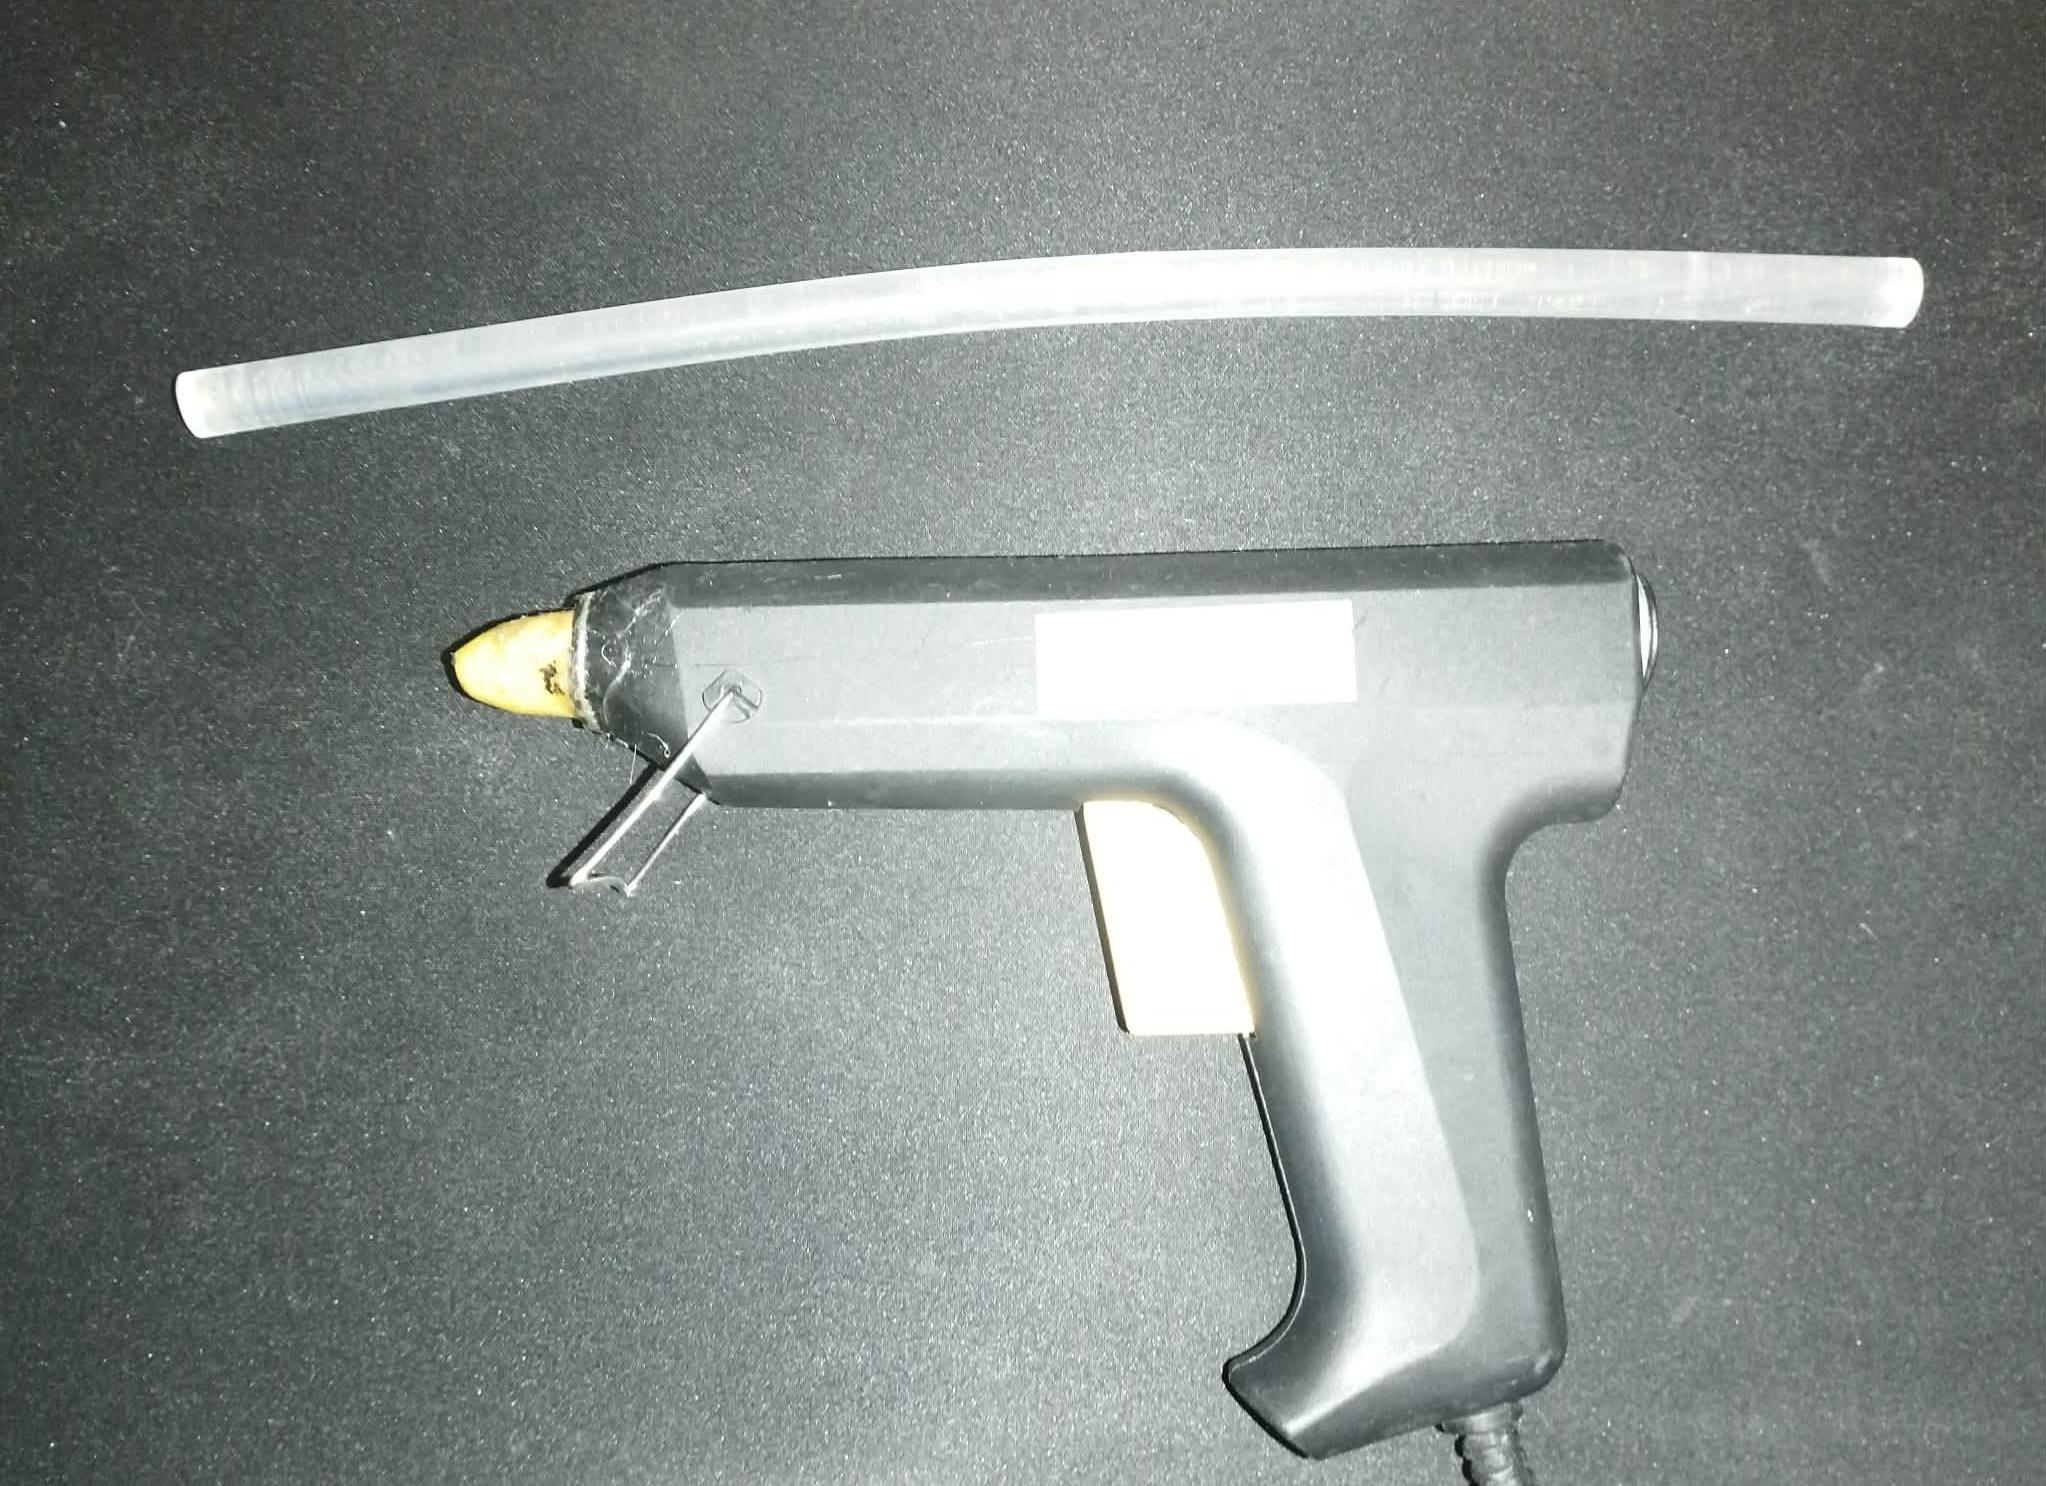
\includegraphics[width=0.5\textwidth]{figures/klej.png}%
 \caption{Pistolet na klej termotopliwy wraz z wkładem}%
 \label{Fig:klej}%
\end{figure}

\begin{figure}[ht]%
 \centering%
 \includegraphics[width=0.5\textwidth]{figures/lutownica.png}%
 \caption{Lutownica, cyna bezołowiowa oraz pasta lutownicza}%
 \label{Fig:lutownica}%
\end{figure}

\subsection{Budowa prototypu robota}

Przed przystąpieniem do realizacji właściwego projektu praktycznego zasadnym etapem procesu inżynierskiego jest wykonanie prototypu, którego celem jest weryfikacja przyjętych założeń projektowych oraz identyfikacja potencjalnych problemów konstrukcyjnych na wczesnym etapie prac.

Celem budowy pierwszej wersji robota było potwierdzenie możliwości realizacji głównego założenia projektowego, jakim było stworzenie autonomicznej konstrukcji mobilnej zdolnej do poruszania się w środowisku oraz omijania przeszkód na podstawie danych pozyskiwanych z czujnika ultradźwiękowego. Na etapie prototypowania pominięto zagadnienia związane z estetyką oraz wysoką precyzją wykonania, takie jak dokładne poziomowanie kół, docelowe rozmieszczenie komponentów czy optymalizacja sposobu ich montażu. Elementy te zostały zaplanowane do dopracowania w finalnej wersji robota.

Podczas projektowania i budowy prototypu przyjęto następujące podstawowe założenia:
\begin{enumerate}
\item Prototyp robota musi umożliwiać realizację funkcji autonomicznego poruszania się oraz skutecznego omijania przeszkód, zgodnie z celem projektu.
\item Rozmieszczenie komponentów na płycie konstrukcyjnej nie może powodować przesunięcia środka ciężkości robota poza geometryczny środek konstrukcji, co mogłoby prowadzić do utraty stabilności oraz pogorszenia jakości manewrów ruchu.
\end{enumerate}

\subsubsection{Lutowanie wyprowadzeń silników}

W pierwszym etapie montażu przeprowadzone zostało łączenie wyprowadzeń silników z kablami (Rys. \ref{Fig:lutowanie1}). Wykonanie tego kroku przed połączeniem silników z podstawą akrylową jest wysoce wskazane ze względu na znacznie większą swobodę wykonywania ruchów lutownicą. 

\begin{figure}[ht]%
 \centering%
 \includegraphics[width=0.8\textwidth]{figures/lutowanie1.png}%
 \caption{Łączenie wyprowadzeń silników z kablami}%
 \label{Fig:lutowanie1}%
\end{figure}

\subsubsection{Montaż silników oraz kół}

Silniki zostały zamocowane symetrycznie względem środka geometrycznego robota, przy rogach platformy (Rys. \ref{Fig:kola}). Ich położenie dobrano w taki sposób, aby oś obrotu kół znajdowała się możliwie blisko tylnej krawędzi płyty nośnej, co zwiększa stabilność robota podczas jazdy oraz ułatwia wykonywanie manewrów skrętu. Do mocowania silników wykorzystano klej termotopliwy, który zapewnia wystarczającą sztywność połączenia przy jednoczesnym zachowaniu możliwości względnie łatwego demontażu w przypadku modyfikacji konstrukcji. Koła zostały osadzone bezpośrednio na wałach silników.

\begin{figure}[ht]%
 \centering%
 \includegraphics[width=0.8\textwidth]{figures/kola.png}%
 \caption{Montaż silników z kołami}%
 \label{Fig:kola}%
\end{figure}

\subsubsection{Montaż mikrokontrolera Arduino Uno}

Płytka Arduino Uno została zamocowana do płyty akrylowej konstrukcji nośnej za pomocą wkrętów dystansowych, co pozwoliło na jej uniesienie ponad powierzchnię podstawy (Rys. \ref{Fig:arduinomontaz}). Takie rozwiązanie minimalizuje ryzyko zwarć elektrycznych, umożliwia swobodny przepływ powietrza pod płytką oraz ułatwia prowadzenie przewodów połączeniowych. Otwory montażowe znajdujące się w narożnikach płytki mikrokontrolera zostały wykorzystane zgodnie z ich przeznaczeniem, co dodatkowo zwiększyło sztywność całego mocowania.

Orientacja mikrokontrolera została dobrana w sposób umożliwiający wygodny dostęp do portu USB oraz złącza zasilania, co znacząco ułatwiało proces programowania oraz diagnostyki układu bez konieczności demontażu robota. Dodatkowo zachowano odpowiednie odstępy pomiędzy mikrokontrolerem a pozostałymi komponentami elektronicznymi, aby zapewnić przejrzystość połączeń.

\begin{figure}[ht]%
 \centering%
 \includegraphics[width=0.8\textwidth]{figures/arduinomontaz.png}%
 \caption{Montaż mikrokontrolera Arduino Uno}%
 \label{Fig:arduinomontaz}%
\end{figure}

\subsubsection{Montaż osłony L293D}

Osłona L293D została zamontowana bezpośrednio na mikrokontrolerze Arduino Uno (Rys. \ref{Fig:l293dmontaz}). Moduł ten został zaprojektowany z myślą o ścisłej współpracy z płytkami Arduino, co umożliwia ich bezpośrednie połączenie bez konieczności stosowania dodatkowych przewodów połączeniowych. Rozmieszczenie wyprowadzeń osłony jednoznacznie determinuje sposób jej instalacji na płytce mikrokontrolera. Podczas montażu należy zwrócić uwagę na prawidłowe dopasowanie złączy pinowych, tak aby gniazda obu płytek pokrywały się ze sobą (Rys. \ref{Fig:l293dlaczenie}).

\begin{figure}[ht]%
 \centering%
 \includegraphics[width=0.8\textwidth]{figures/l293dmontaz.png}%
 \caption{Montaż osłony L293D}%
 \label{Fig:l293dmontaz}%
\end{figure}

\begin{figure}[ht]%
 \centering%
 \includegraphics[width=0.8\textwidth]{figures/l293dlaczenie.png}%
 \caption{Sposób łączenia płytki Arduino Uno z L293D}%
 \label{Fig:l293dlaczenie}%
\end{figure}

\subsubsection{Montaż osłony L293D}

\section{Część Praktyczna/kodowa - zmień nazwę}
\clearpage

\addcontentsline{toc}{section}{Literatura}

\begin{thebibliography}{99}

\bibitem{ifr2023}
International Federation of Robotics:
World Robotics 2023 – Service Robots.
IFR, Frankfurt am Main, 2023.

\bibitem{monk2016}
Monk S.:
Programming Arduino: Getting Started with Sketches.
McGraw-Hill Education, New York, 2016.

\bibitem{siegwart2011}
Siegwart R., Nourbakhsh I. R., Scaramuzza D.:
Introduction to Autonomous Mobile Robots.
MIT Press, Cambridge, 2011.

\bibitem{arduino2022}
Arduino:
Arduino Uno Rev3 – Technical Documentation.
Arduino SA, 2022.

\bibitem{elecfreaks}
Cytron Technologies:
HC-SR04 Ultrasonic Sensor User Manual.
Dokumentacja techniczna, 2013.

\bibitem{cytron2018}
Adafruit Industries:
Adafruit Motor Shield.
Dokumentacja techniczna, 2018.

\bibitem{jones1999}
Jones J. L., Flynn A. M.:
Mobile Robots: Inspiration to Implementation.
A K Peters, Natick, 1999.

\bibitem{horowitz2015}
Horowitz P., Hill W.:
The Art of Electronics.
Cambridge University Press, Cambridge, 2015.

\bibitem{educationalRoboticsOverview}
Alimisis D.:
Educational Robotics: Open Questions and New Challenges.
Themes in Science and Technology Education, Vol. 6, No. 1, 2013, s. 63–71.

\bibitem{campionDifferentialDrive}
Campion G., Bastin G., D’Andrea-Novel B.:
Structural properties and classification of kinematic and dynamic models of wheeled mobile robots.
IEEE Transactions on Robotics and Automation, Vol. 12, No. 1, 1996, s. 47–62.

\bibitem{reactiveNavigation}
Arkin R. C.:
Behavior-Based Robotics.
MIT Press, Cambridge, 1998.

\bibitem{ultrasonicSensorComparison}
Kurniawan A., Hadiyoso S.:
Performance Comparison of Ultrasonic Sensors for Obstacle Detection.
International Journal of Engineering Research, Vol. 7, No. 4, 2018, s. 210–215.

\bibitem{sensorFiltering}
Welch G., Bishop G.:
An Introduction to the Kalman Filter.
University of North Carolina at Chapel Hill, 2006.

\bibitem{slamOverview}
Durrant-Whyte H., Bailey T.:
Simultaneous Localization and Mapping: Part I.
IEEE Robotics \& Automation Magazine, Vol. 13, No. 2, 2006, s. 99–110.

\bibitem{thrunSLAM}
Thrun S., Burgard W., Fox D.:
Probabilistic Robotics.
MIT Press, Cambridge, 2005.

\bibitem{mobileRoboticsClassification}
Borenstein J., Everett H. R., Feng L.:
Where am I? Sensors and Methods for Mobile Robot Positioning.
University of Michigan, 1996.

\bibitem{borensteinMobilePlatforms}
Borenstein J.:
Control and kinematic design of multi-degree-of-freedom mobile robots.
IEEE Transactions on Robotics and Automation, Vol. 14, No. 2, 1998, s. 315–322.

\bibitem{leggedRobotsControl}
Raibert M.:
Legged Robots That Balance.
MIT Press, Cambridge, 1986.

\bibitem{advancedRobotArchitectures}
Brooks R. A.:
A Robust Layered Control System for a Mobile Robot.
IEEE Journal of Robotics and Automation, Vol. 2, No. 1, 1986, s. 14–23.

\bibitem{robotKinematicsDynamics}
Siciliano B., Sciavicco L., Villani L., Oriolo G.:
Robotics: Modelling, Planning and Control.
Springer, London, 2010.

\bibitem{mobileRobotNonlinearModel}
Canudas-de-Wit C., Siciliano B., Bastin G.:
Theory of Robot Control.
Springer, London, 1996.

\bibitem{nonholonomicConstraints}
Bloch A. M.:
Nonholonomic Mechanics and Control.
Springer, New York, 2003.

\bibitem{embeddedMotorControl}
Kenjo T.:
Stepping Motors and Their Microprocessor Controls.
Oxford University Press, Oxford, 1994.

\bibitem{educationalRobotsModeling}
Eguchi A.:
Educational Robotics for Promoting 21st Century Skills.
Journal of Automation, Mobile Robotics \& Intelligent Systems, Vol. 8, No. 1, 2014, s. 5–11.

\bibitem{lavallePlanningAlgorithms}
LaValle S. M.:
Planning Algorithms.
Cambridge University Press, Cambridge, 2006.

\bibitem{motorPowerSupplyIssues}
Erickson R. W., Maksimović D.:
Fundamentals of Power Electronics.
Springer, New York, 2020.


\end{thebibliography}



\clearpage

\makesummary

\end{document} 
